\documentclass{beamer}
\usepackage{graphicx}
\usefonttheme[onlymath]{serif}
\usepackage[utf8]{inputenc}
\renewcommand{\vec}[1]{\mathbf{#1}}
 \newcommand{\grad}{\nabla}
\newcommand{\partiald}[2]{\frac{\partial {#1} }{\partial {#2}}}
%Information to be included in the title page:
\title{Rossby Waves}
\author{Group 1}
\institute{MPE CDT }
\date{\today}
\begin{document}
	
	\frame{\titlepage}
 \begin{frame}
\frametitle{Quasi stationary synoptic Rossby waves high amplitude during weather events }
\framesubtitle{by Petoukhov, Rahmstorf, Pteri and Schellnhuber 2013}
\begin{itemize}
	\item Investigated physical model of quasi resonance effect.
	\item Forced wave trapping a free wave.
	\item Amplification of pressure system.
	\item Extreme weather results.
\end{itemize}
\centering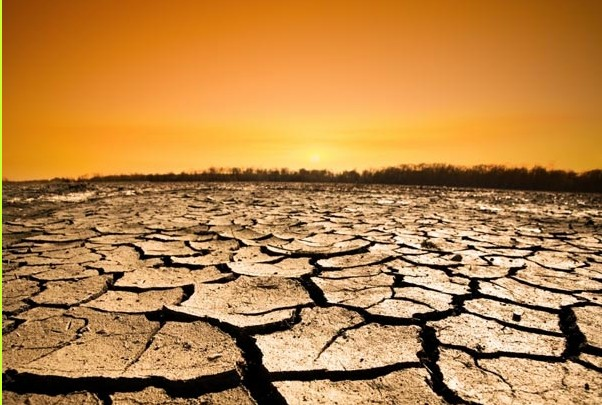
\includegraphics[height=0.4\textheight]{drought}

\end{frame}
\begin{frame}
\frametitle{Amplified mid-latitude planetary waves favour particular regional weather extremes}
\framesubtitle{ 
by Screen and Simmonds }
\begin{itemize}
\item Looked at distribution of quasi resonance events.
\item Examined links between temperature and precipitation anomalies and abnormal quasi stationary wave amplitude from 1979 to 2012.

\end{itemize}
\centering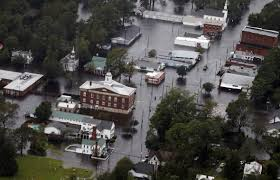
\includegraphics[height=0.4\textheight]{flood}
\end{frame}

\begin{frame}
\frametitle{40 most extreme temperature and precipitation events in the mid latitudes between 1979 and 2012.}
\centering
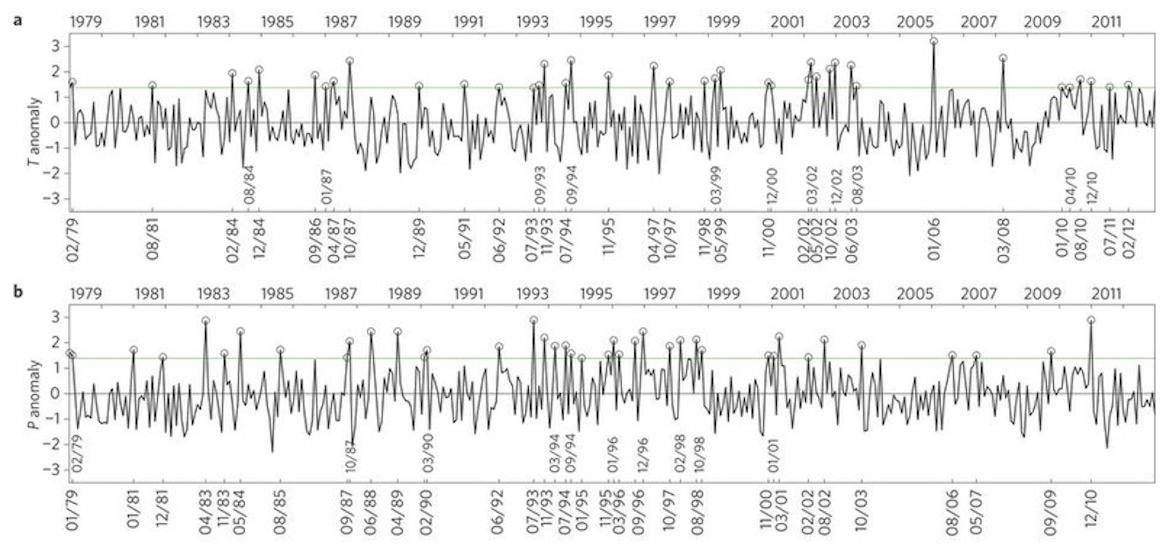
\includegraphics[scale=0.53]{Cathie1}


\end{frame}
\begin{frame}
\frametitle{Anomalies: Prolonged periods over a large area}
\begin{tabular}{c c}
\huge{Temperature}&\vspace{5pt}\\

\Large{Positive: abnormally high}	&	\Large{	Negative: abnormally low}\vspace{20pt}\\

\huge{Precipitation}&\vspace{5pt}\\
\Large{Positive: abnormally wet} &		\Large{	Negative: abnormally dry}\\
\end{tabular}


\end{frame}
\begin{frame}
\frametitle{Mid latitude regions of the Northern hemisphere examined}
\centering
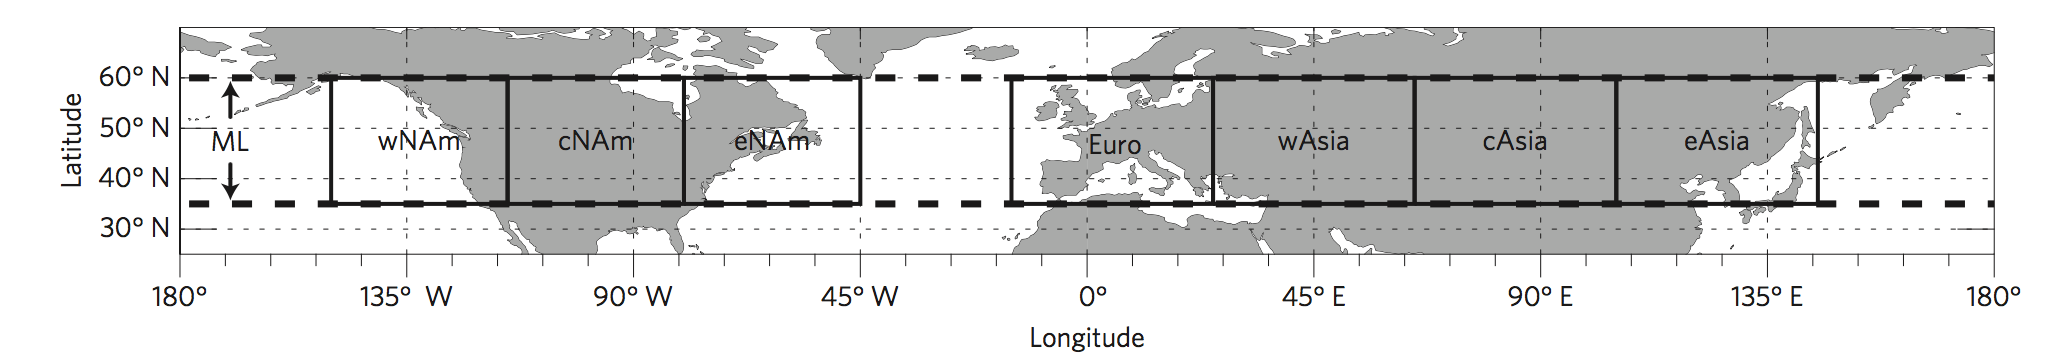
\includegraphics[scale=0.3]{Cathie2}
\end{frame}
\begin{frame}
\frametitle{Charts to show the normalized amplitude anomalies for each extreme temperature event, in order of severity of weather, taking the most extreme events on the left.}
\centering
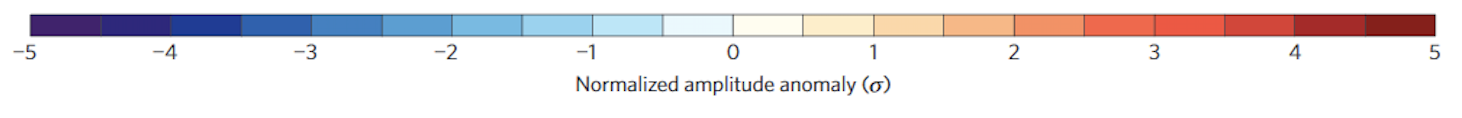
\includegraphics[scale=0.4]{Cathie4}
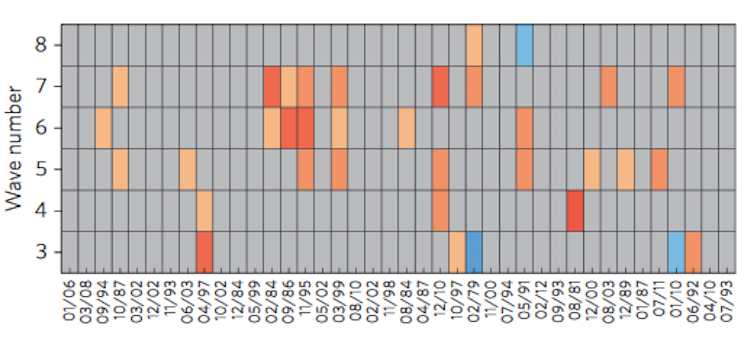
\includegraphics[scale=0.7]{Cathie5}
\end{frame}
\begin{frame}
\frametitle{Charts to show the normalized amplitude anomalies for each extreme precipitation event, in order of severity of weather, taking the most extreme events on the left.}
\centering
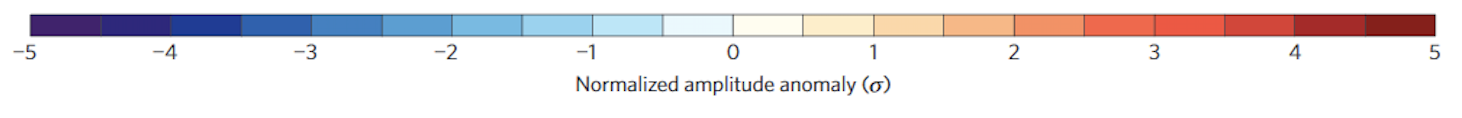
\includegraphics[scale=0.4]{Cathie4}
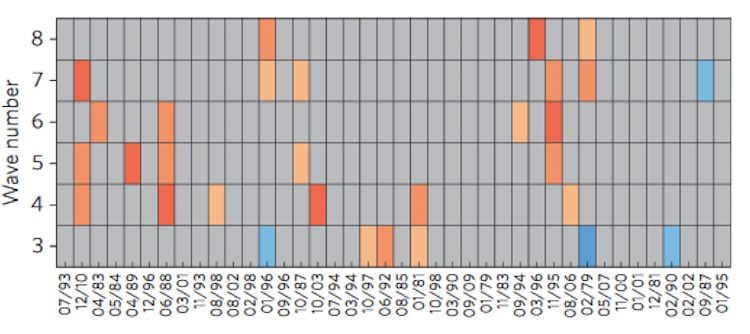
\includegraphics[scale=0.7]{Cathie6}
\end{frame}
\begin{frame}
\frametitle{Distributions comparing observed frequency of anomalous amplitudes of baroclinic Rossby waves during periods of extreme weather and the distributions expected from climatology across each examined region.}
\centering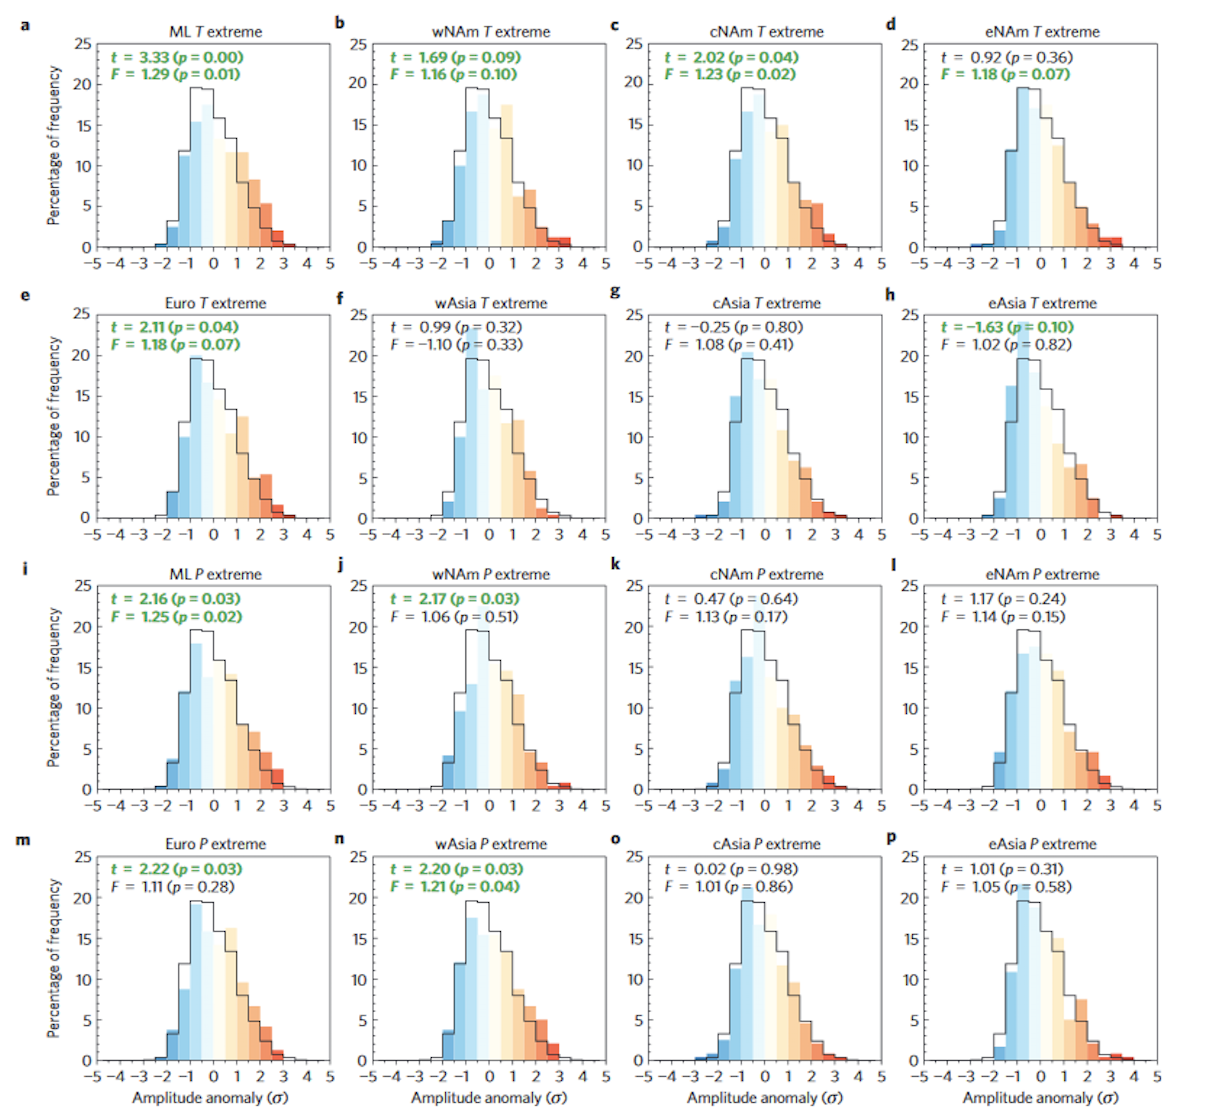
\includegraphics[scale=0.3]{Cathie7}
\end{frame}
\begin{frame}
\frametitle{Future Forecast}
\centering
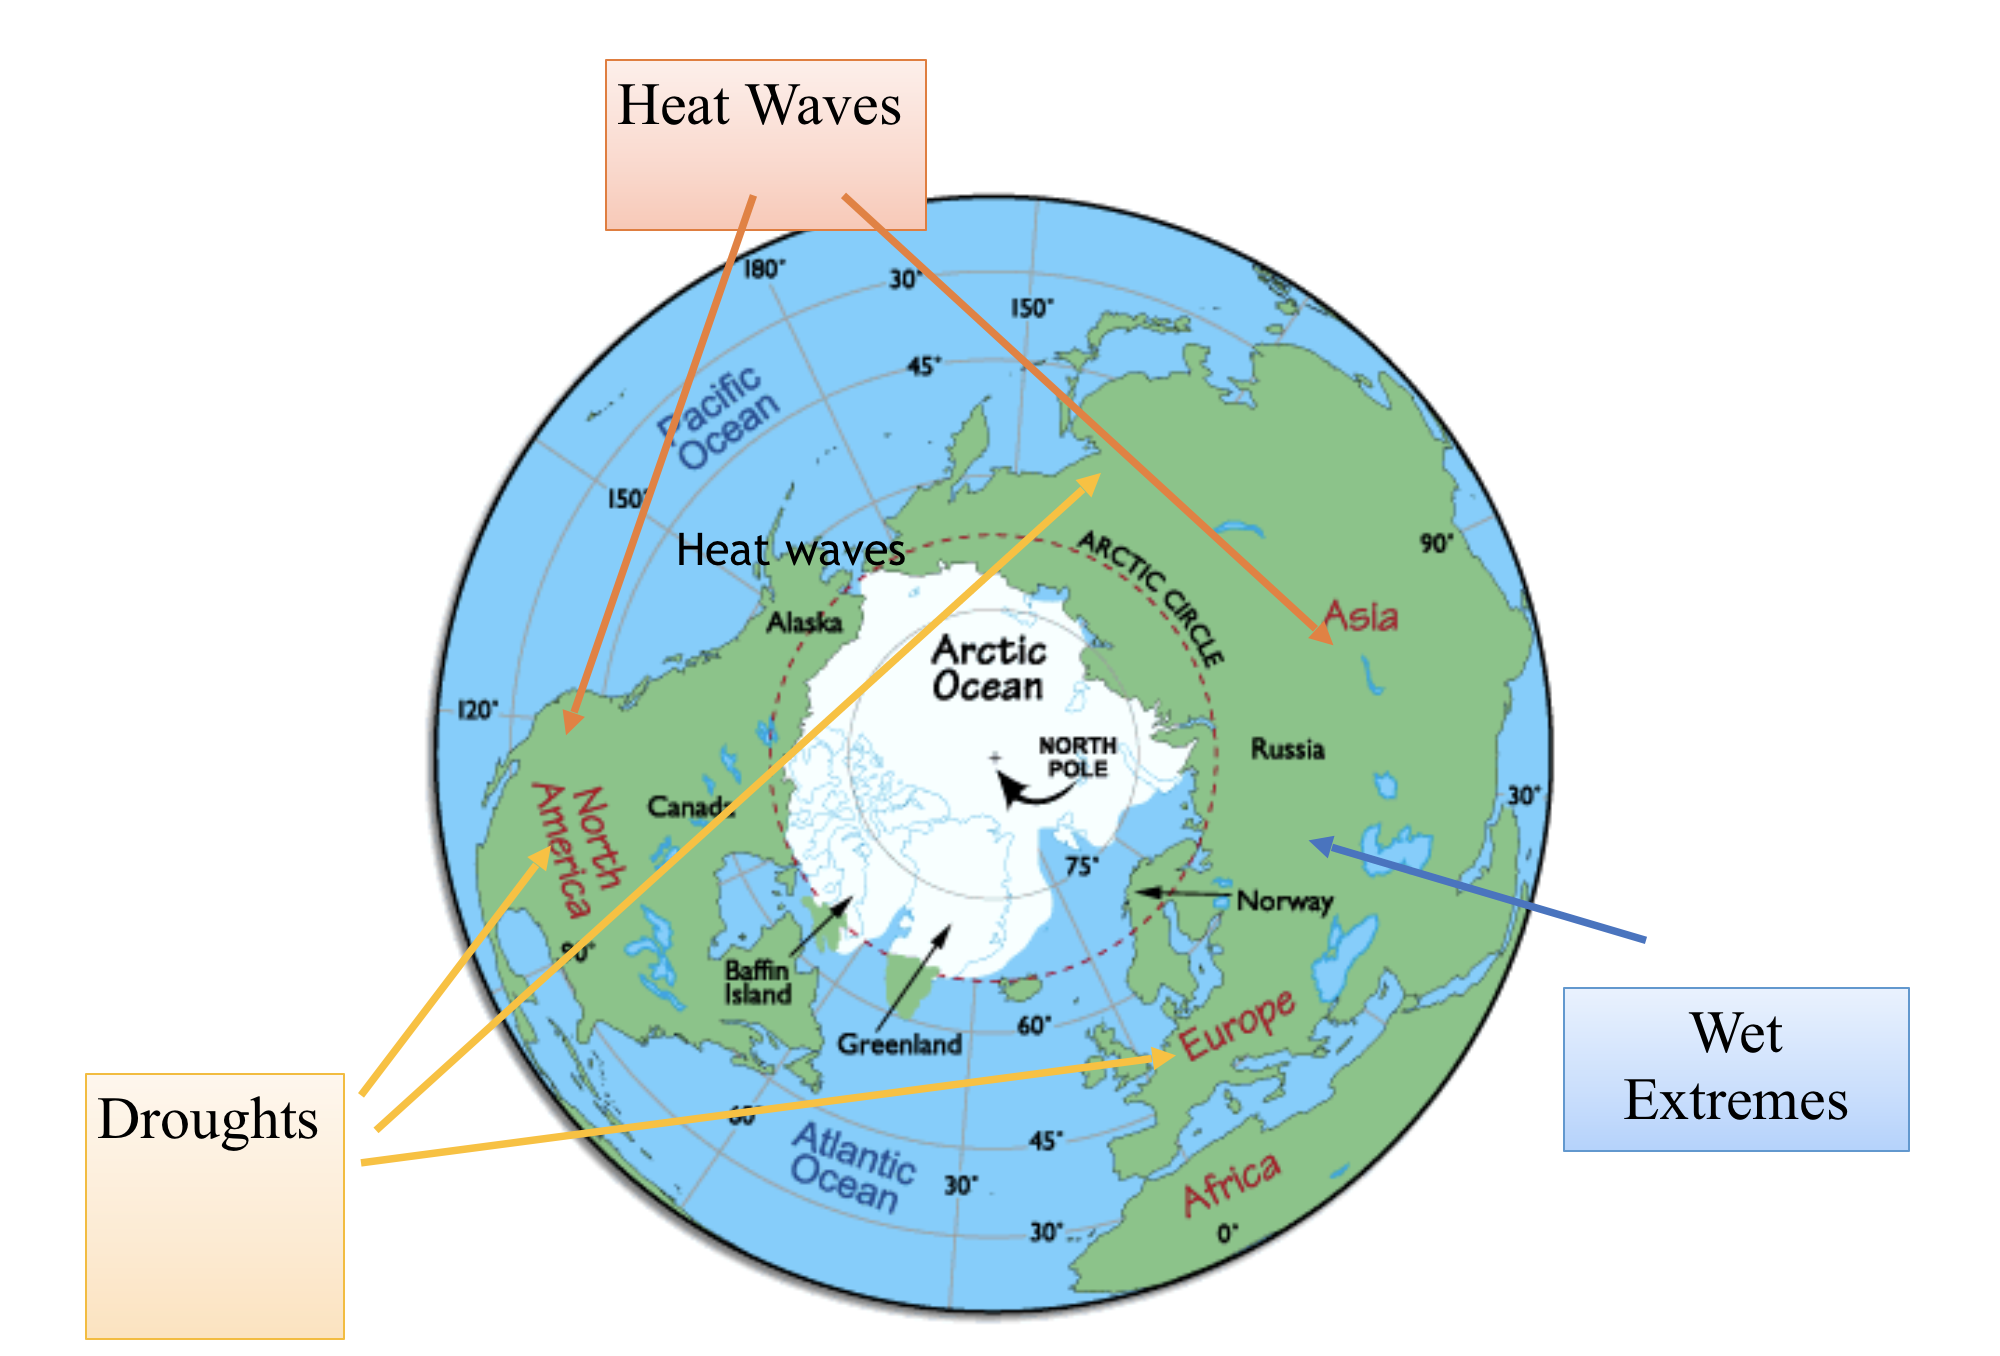
\includegraphics[scale=0.3]{Cathie8}

\end{frame}
\end{document}